\chapter{Evaluation und Validierung}

\section{Versuchsaufbau und Testbedingungen}

\section{Erkennungsgenauigkeit}

\section{Konfusionsmatrix und klassenbezogene Ergebnisse}

\begin{longtable}{|p{0.4\textwidth}|p{0.2\textwidth}|}
    \caption{Trainingsergebnisse des Klassifizierungsmodells}
    \label{tab:trainingsergebnisse} \\
    \hline
    \textbf{Metrik} & \textbf{Wert} \\
    \hline
    \endfirsthead
    \hline
    \textbf{Metrik} & \textbf{Wert} \\
    \hline
    \endhead
    \hline
    \multicolumn{2}{r}{\texttt{Fortsetzung auf nächster Seite}} \\
    \endfoot
    \hline
    \endlastfoot
    Trainingsgenauigkeit        & 98,34\,\% \\
    \hline
    Validierungsgenauigkeit     & 99,21\,\% \\
    \hline
    Finaler Trainingsverlust    & 0,0754 \\
    \hline
    Finaler Validierungsverlust & 0,0319 \\
    \hline
\end{longtable}

\begin{figure}[htbp]
    \centering
    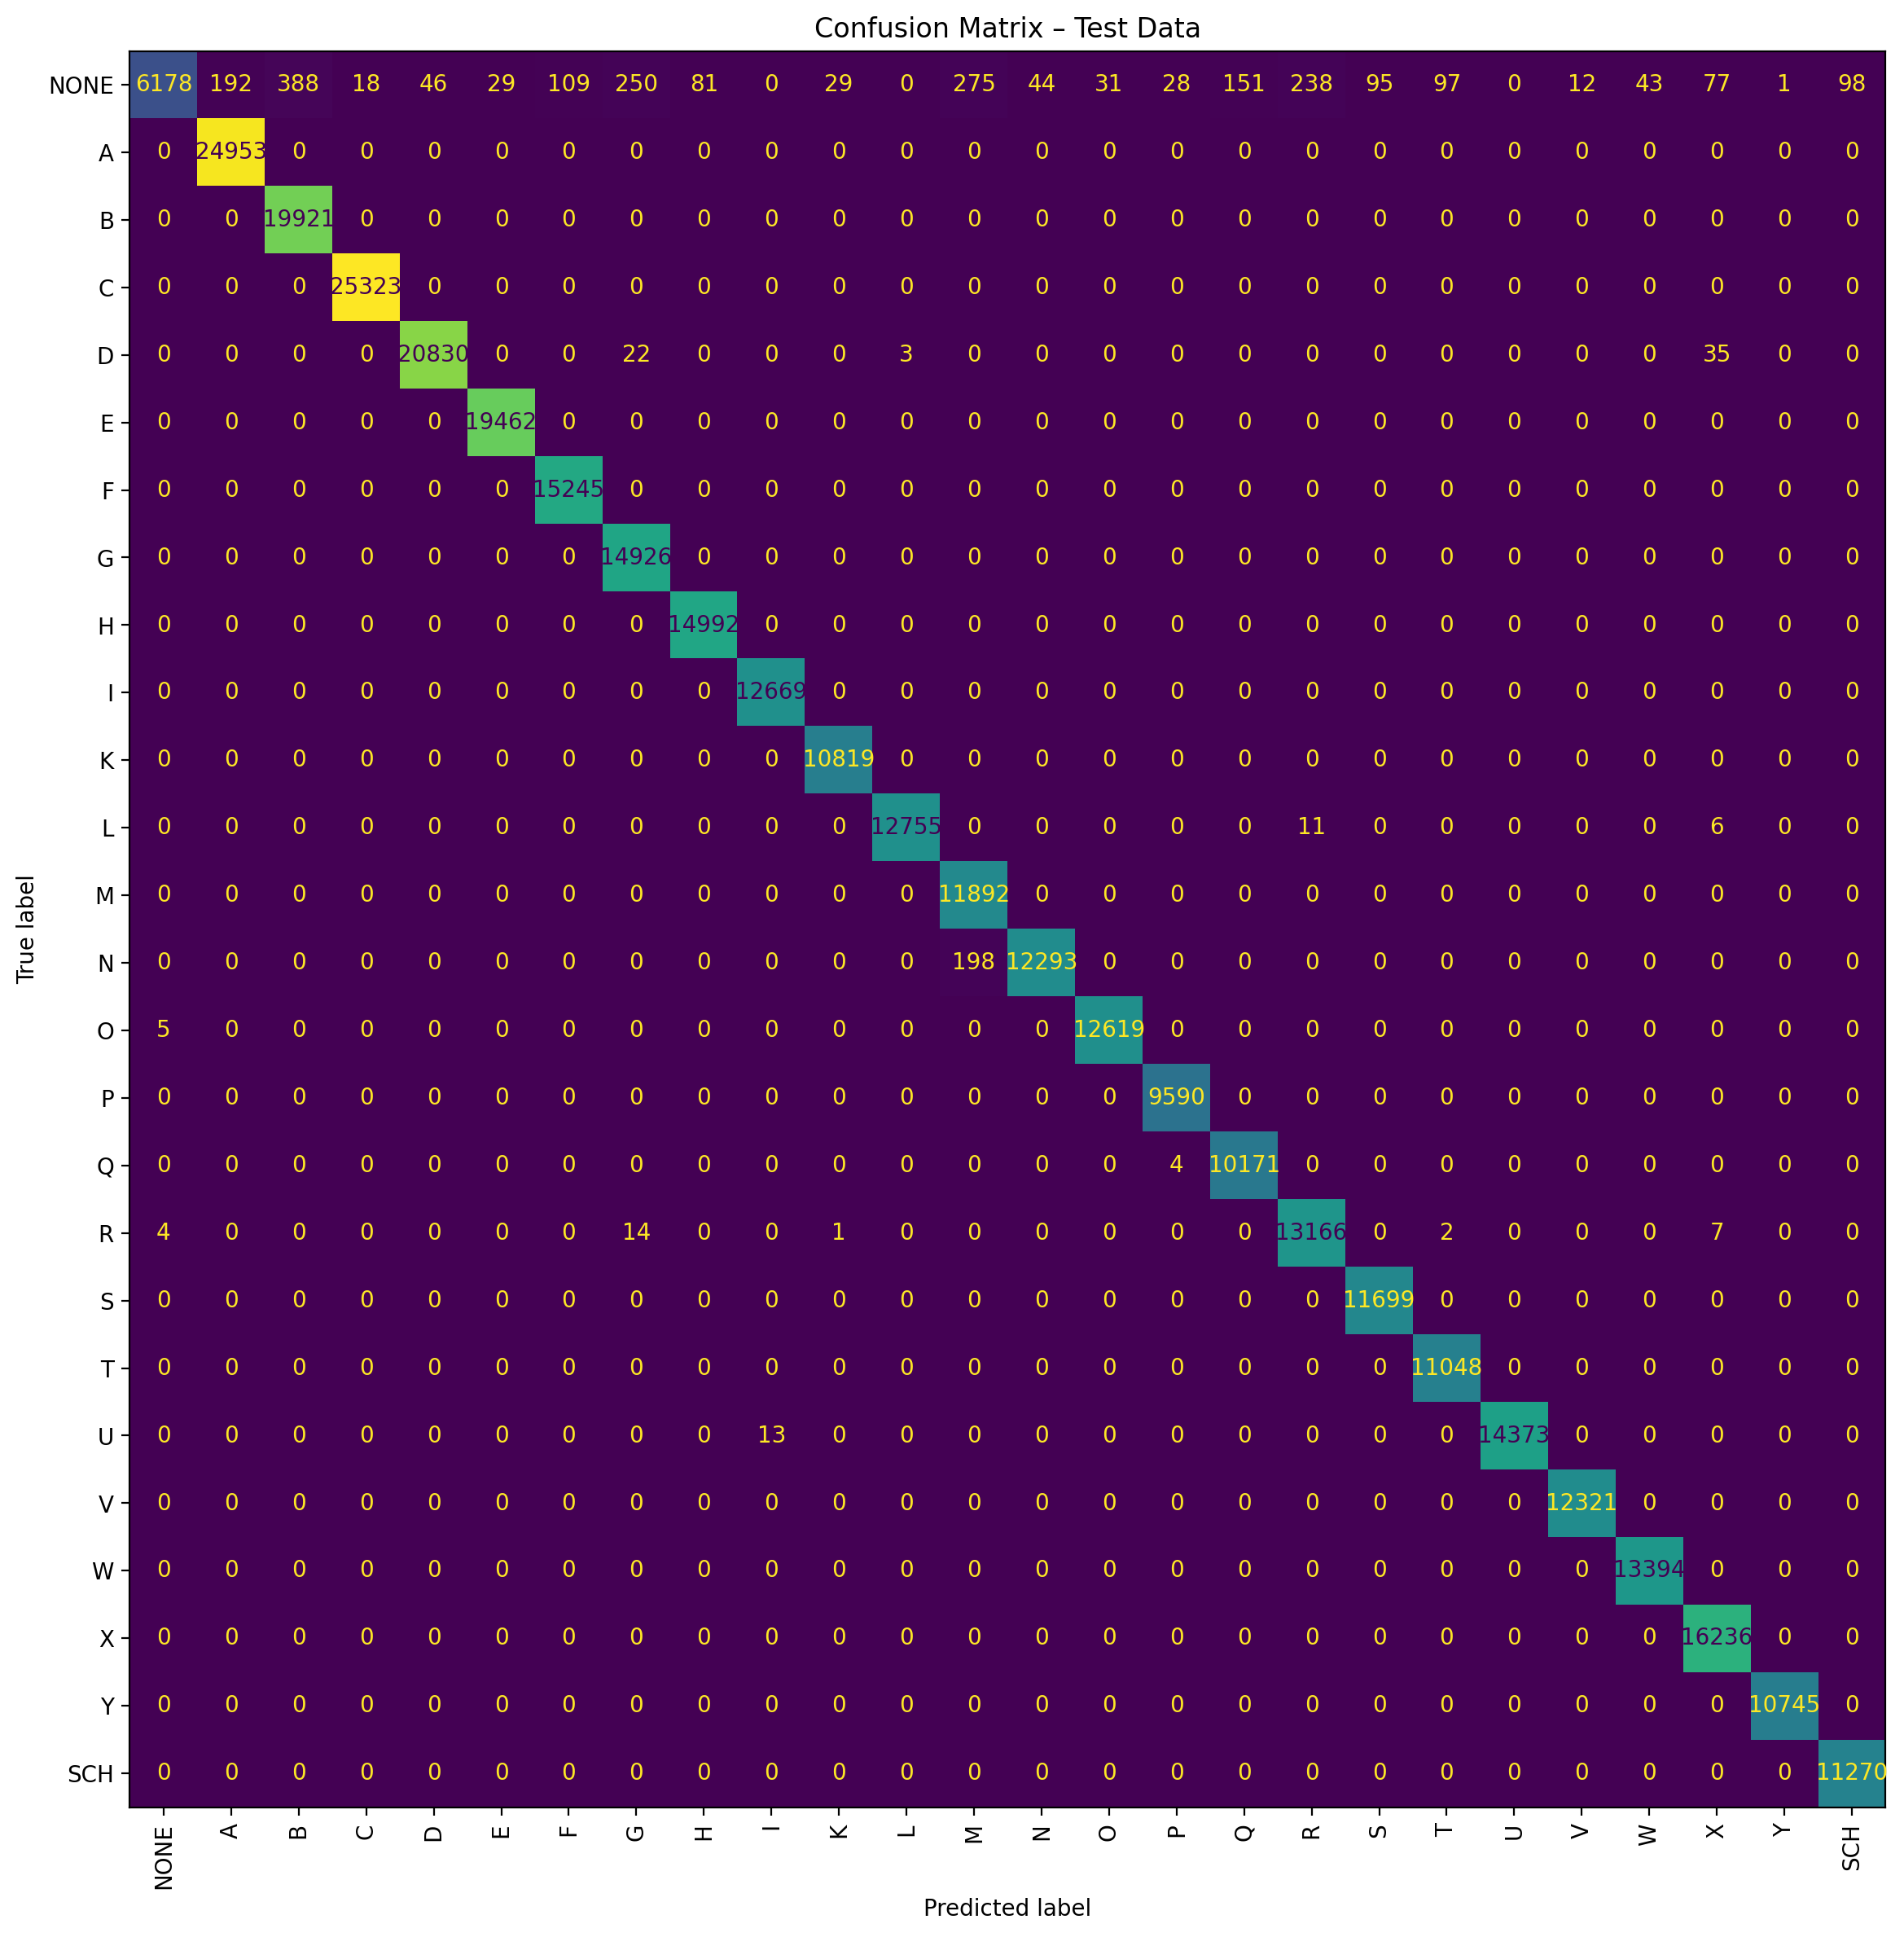
\includegraphics[width=0.6\textwidth]{material/figures/confusion_matrix.png}
    \caption{Konfusionsmatrix}
    \label{fig:confusion-matrix}
\end{figure}

\begin{figure}[htbp]
    \centering
    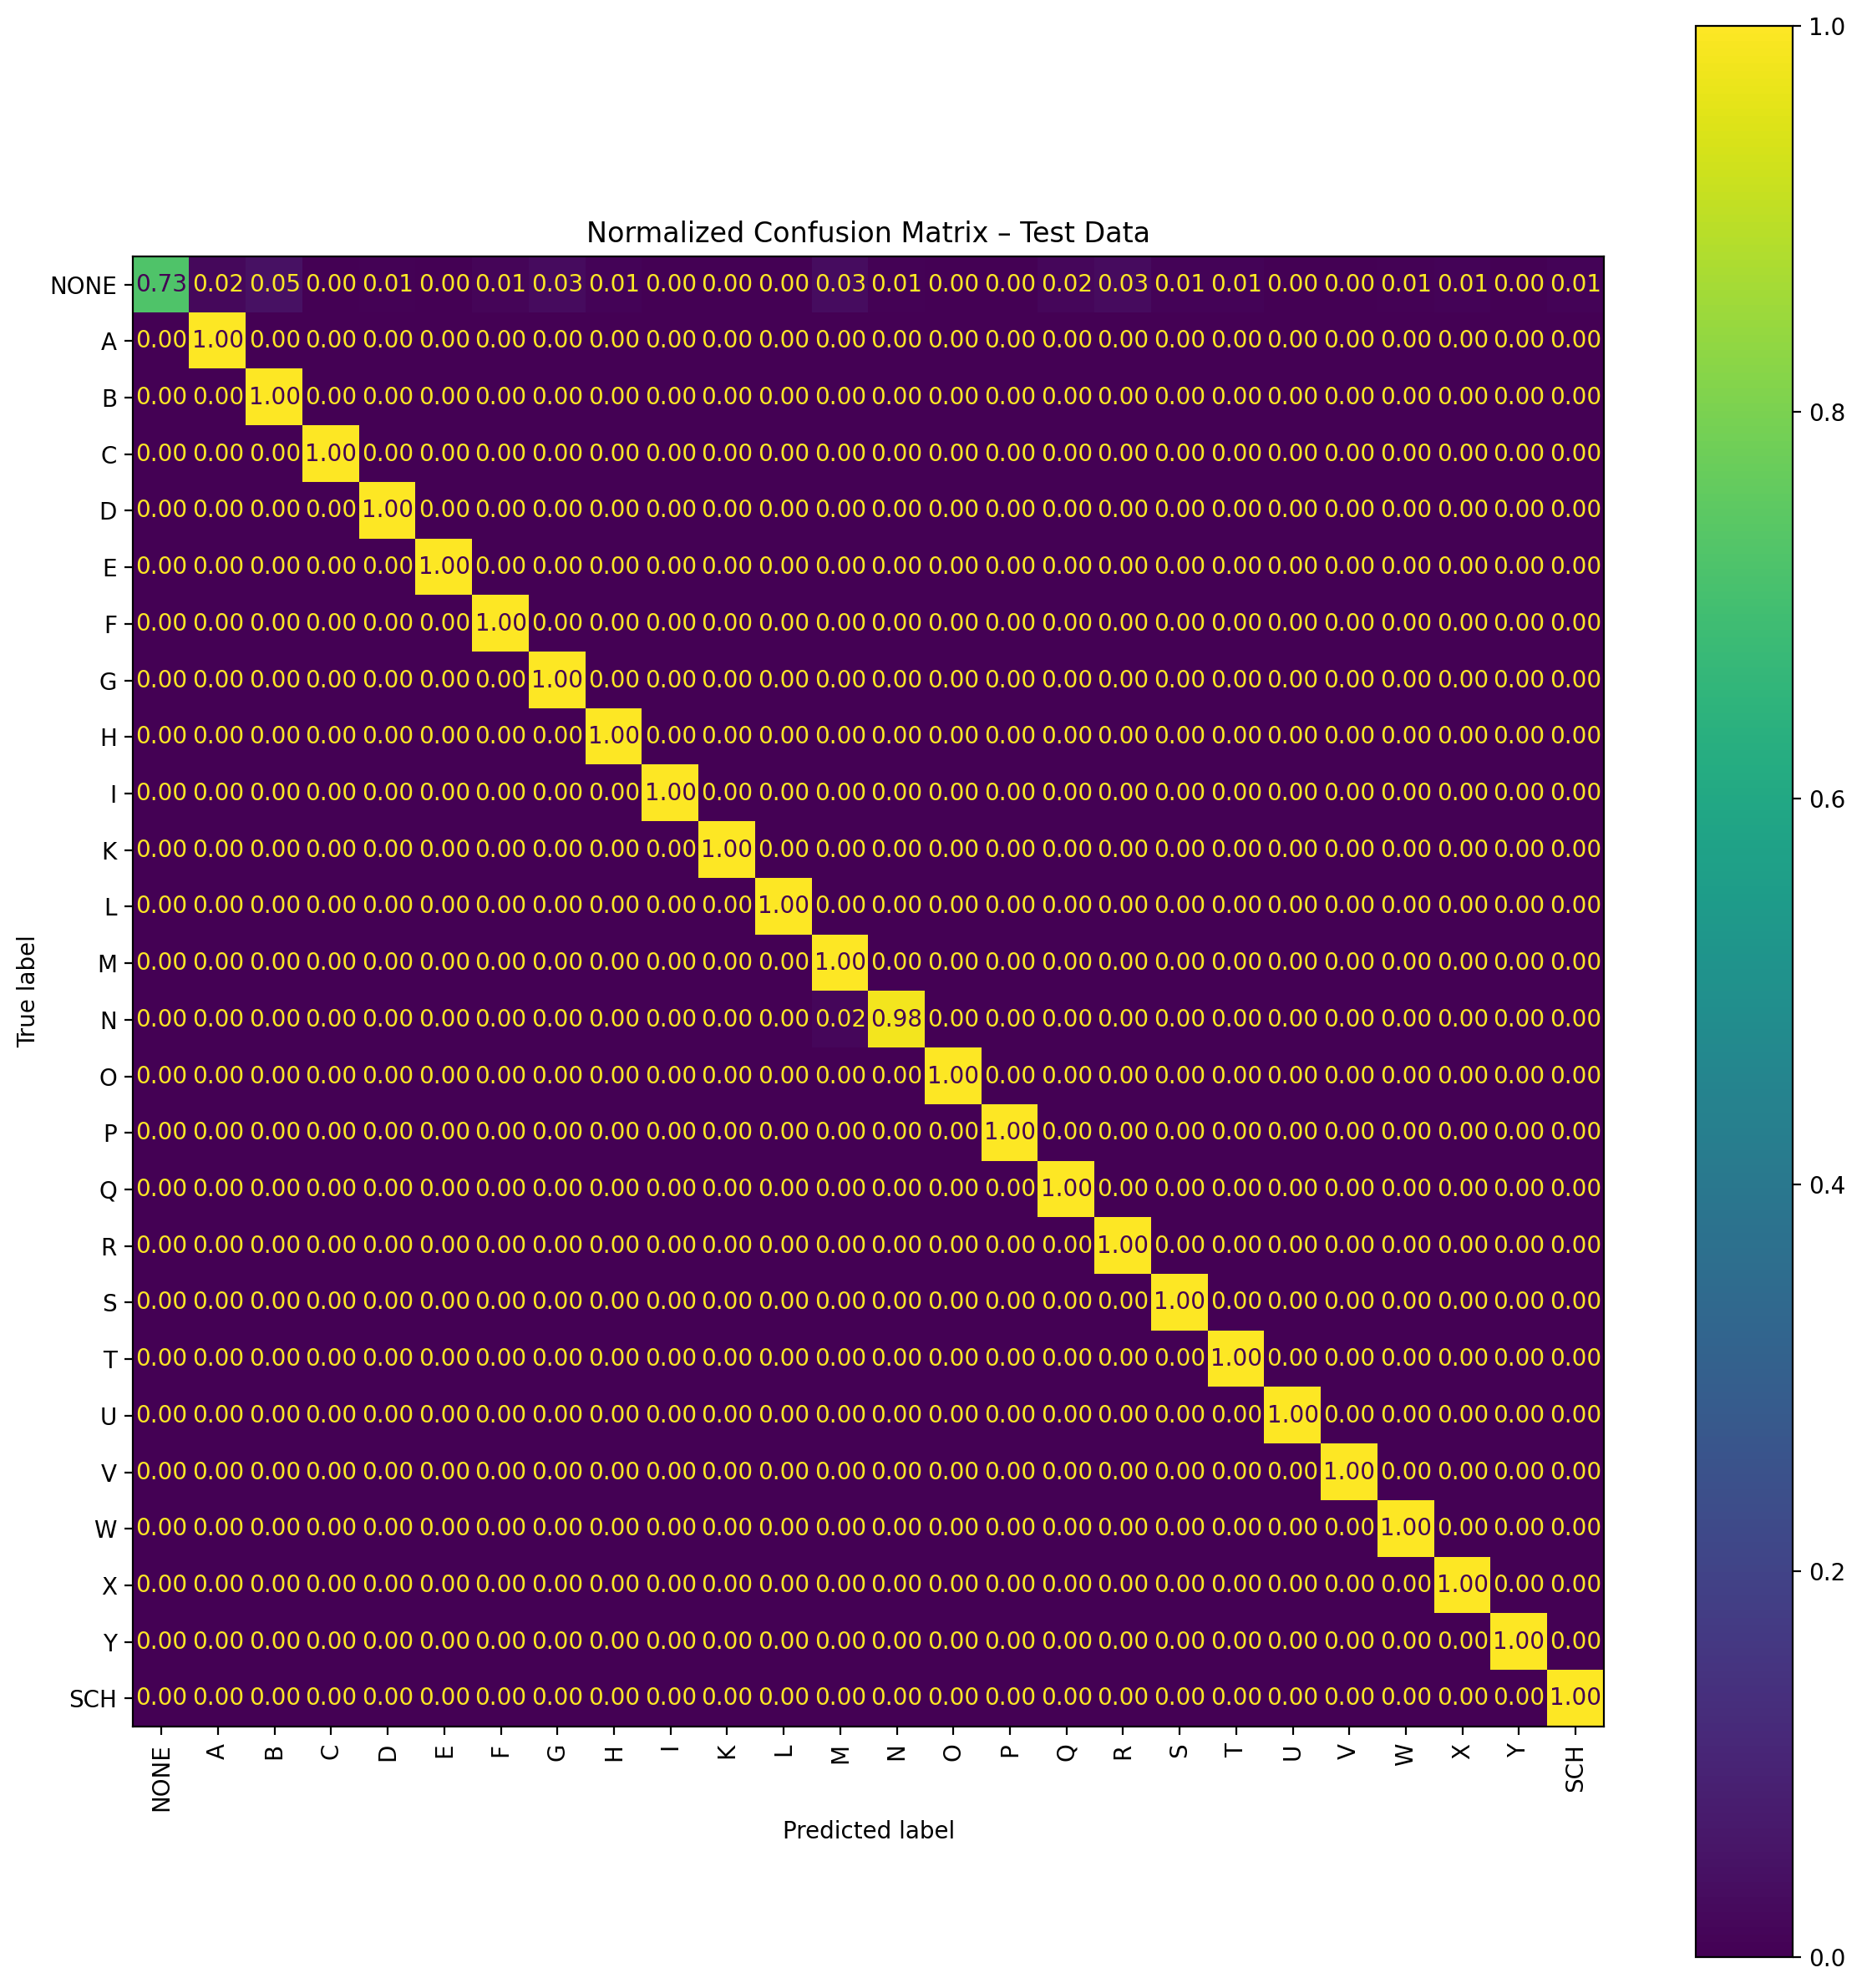
\includegraphics[width=0.6\textwidth]{material/figures/confusion_matrix_normalized.png}
    \caption{Normalisierte Konfusionsmatrix}
    \label{fig:confusion-matrix-normalized}
\end{figure}

Das Modell zeigt keine Anzeichen von Overfitting: Der Validierungsverlust sinkt kontinuierlich über alle 20 Epochen.

\section{Einfluss von Beleuchtung und Hintergrund}
\section{Inferenzlatenz und Ende-zu-Ende-Latenz}
\section{Bildrate und Datendurchsatz}
\section{Speicher- und Ressourcenverbrauch}
\section{Abgleich mit den definierten Anforderungen}
